
\chapter{引言}


\section{研究背景}

\subsection{Linux的开发模式}

\begin{figure}[H]
\centering
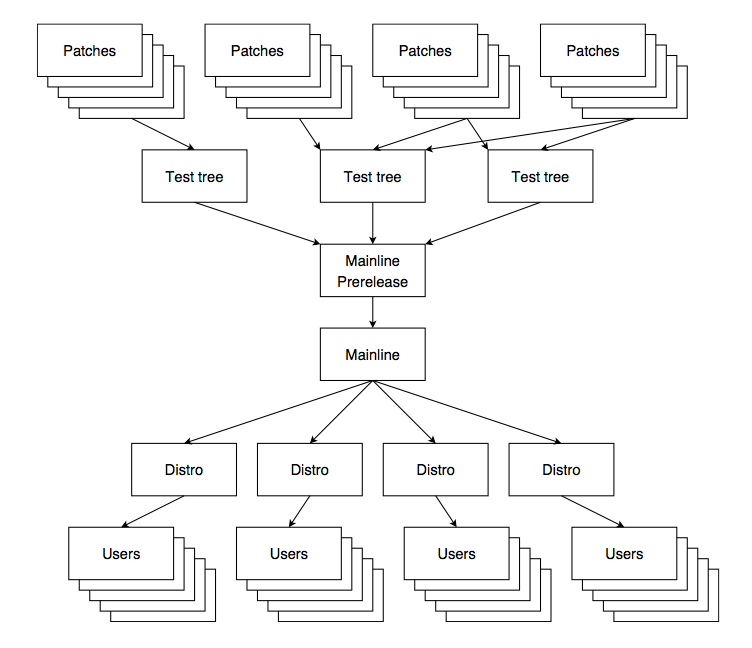
\includegraphics[width=10cm]{linux_kernel_change_flow}
\caption{Linux内核开发模式}
\label{fig:linux_kernel_change_flow}
\end{figure}

\subsection{Linux的开发特点}

随着Linux内核开发的全球化,Linux开发的步伐也逐渐加快,开发的规模也逐渐扩大,目前内核开发大致具有以下的特点:

\begin{enumerate}
\item 越来越多的新功能被添加到内核中来,导致内核的结构越来越复杂
\item 内核的复杂结构使得任何一点改动对内核性能造成影响的可能性加大
\item Linux内核进行官方测试的间隔一般比较大(一般旨在有新版本发布的时候才会进行比较完整的测试)
\item 一旦发现版内核中出现性能回退的问题,这个问题就会随着各大Linux发行版扩散到广大的用户当中
\end{enumerate}

\section{课题目标}

正如研究背景所述,目前Linux内核的开发具有比较鲜明的特点,而且Linux作为一个操作系统内核,也具有一点的特殊性,因此,很有必要设计并实现出一套与Linux内核相适应的性能测试框架,方便Linux的开发者们更加方便地进行性能回退问题的管理和处理。

本课题的目的就是设计并实现一套能够进行Linux性能测试并具有如下特征的框架(系统):

\begin{enumerate}
\item 较快并准确进行Linux性能测试
\item 在出现性能回退之后,多次运行进行问题确认
\item 确认性能回退之后,能够最快地定位到出现问题的代码
\item 在定位到问题代码之后,将相关的测试数据及出现问题的代码通知给相关代码的作者
\end{enumerate}